\documentclass[12pt,a4paper]{article}
\usepackage{graphicx} % Required for inserting images
\setlength{\topmargin}{0.0in}
\setlength{\oddsidemargin}{0.33in}
\setlength{\textheight}{9.0in}
\setlength{\textwidth}{6.0in}
\renewcommand{\baselinestretch}{1.25}


\usepackage{hyperref}
% \usepackage[utf8]{inputenc}
% \usepackage[T1]{fontenc}
\usepackage{float}
\usepackage{enumitem}
\usepackage{amsmath}
\usepackage{amssymb}
\usepackage{amsthm}
\usepackage{tikz}
\usepackage{amsfonts}
\usepackage{graphicx}
\usepackage{subcaption}
\usepackage{caption}
\usepackage{booktabs}
\usepackage{graphicx}
\newcommand{\dv}[2]{\frac{\mathrm{d} #1}{\mathrm{d} #2}}
\usepackage{caption}
\captionsetup[figure]{font=small} 
% \captionsetup[table]{font=small}
\usepackage[capitalize,nameinlink]{cleveref}
\usepackage{mathtools}
\newcommand{\defeq}{\vcentcolon=}
\newcommand{\eqdef}{=\vcentcolon}



\newtheoremstyle{boldthm}
  {3pt}        % space above
  {3pt}        % space below
  {\itshape}   % body font
  {}           % indent
  {\bfseries}  % theorem head font
  {.}          % punctuation
  {.5em}       % space after theorem head
  {\thmname{#1}\thmnumber{ #2}\thmnote{ \textbf{(#3)}}}

\newtheoremstyle{bolddefn}
  {3pt}
  {3pt}
  {\itshape} 
  {}
  {\bfseries}
  {.}
  {.5em}
  {\thmname{#1}\thmnumber{ #2}\thmnote{ \textbf{(#3)}}}


\theoremstyle{boldthm}
\newtheorem{theorem}{Theorem}[section]
\newtheorem{corollary}[theorem]{Corollary}
\newtheorem{lemma}[theorem]{Lemma}
\newtheorem{proposition}[theorem]{Proposition}

\theoremstyle{bolddefn}
\newtheorem{definition}[theorem]{Definition}
\newtheorem{example}[theorem]{Example}
\newtheorem{remark}[theorem]{Remark}

% Define environments
% \newtheorem{theorem}{Theorem}
% \newtheorem{definition}{Definition}
% \newtheorem{lemma}{Lemma}
% \newtheorem{corollary}{Corollary}


\title{Finite Elements for Computing Spectra}
\author{Maggie McCarthy}
\date{May 2026}

\begin{document}

\maketitle

\section{Laplace Eigenvalue Problem}

\subsection{In One Dimension}


Consider $\Omega = (0, \pi).$ We want to find the eigenvalues, $\lambda,$ and the eigenfunctions, $u \ne 0,$ such that
\begin{equation}\label{strong 1D}
\begin{aligned}
     -u''(x) &= \lambda u(x), \qquad \text{for} \qquad x \in \Omega,\\
     u(0) &=u(\pi) = 0.
\end{aligned}
\end{equation}
% where,
% $$ u(0)=u(\pi) = 0.$$
It is well-known that $\lambda = 1, 4, 9, 16, \dots$ and $u(x) = \sin(kx)$ for $k \in \mathbb{N}_1.$


Let $V = H_0^1(\Omega).$ Multiplying \eqref{strong 1D} by a $v \in V$ and integrating by parts, we obtain the variational formulation: find $\lambda \in \mathbb{R}$ and a nonvanishing $u \in V$ such that
\begin{equation}
    \int_{0}^{\pi} u'(x) v'(x) \, dx = \lambda \, \int_0^{\pi} u(x) v(x) \, dx
\end{equation}
for all $v \in V.$

To discretize the infinite-dimensional problem, we consider a finite-dimensional subspace, $V_h = \text{span}\{\phi_1, \phi_2, \dots, \phi_N\} \subset V.$ Then, in this subspace, we look for discrete eigenvalues, $\lambda_h \in \mathbb{R},$ and nonvanishing eigenfunctions, $u_h \in \mathbb{R},$ such that
\begin{equation}
    \int_{0}^{\pi} u_h'(x) v'(x) \, dx = \lambda_h \, \int_0^{\pi} u_h(x) v_h(x) \, dx
\end{equation}
for all $v \in V_h.$

Using the basis for $V_h,$ the discrete variational problem can be written as the generalized eigenvalue problem
$$ Ax = \lambda M x, $$
Here, the stiffness matrix is $A = \{a_{ij}\}_{i,j}^N,$ where
\begin{equation}
a_{ij}
=
\int_0^\pi \varphi_j'(x)\varphi_i'(x)\,dx
\end{equation}
Similarly, the mass matrix is $M = \{m_{ij}\}_{i,j}^N,$ where
\begin{equation}
m_{ij}
=
\int_0^\pi \varphi_j(x)\varphi_i(x)\,dx
\end{equation}


Take a uniform partition of $[0, \pi]$ with spacing $h.$ Let $V_h$ be the space of continuous piecewise linear polynomials vanishing at the endpoints of the interval (standard conforming $P^1$ elements). Then, the associated stiffness and mass matrices are
\begin{equation}
a_{ij}
=
\frac{1}{h}
\begin{cases}
2, & i=j,\\
-1, & |i-j|=1,\\
0, & \text{otherwise},
\end{cases}
\qquad
m_{ij}
=
h
\begin{cases}
4/6, & i=j,\\
1/6, & |i-j|=1,\\
0, & \text{otherwise},
\end{cases}
\end{equation}
respectively.

In this case, we can compute the explicit eigenmodes. In particular, given a $k \in \mathbb{N}_1,$ the $k$th eigenspace is generated by the interpolant of the continuous solution, i.e.,
\begin{equation}
u_h^{(k)}(ih) = \sin(kih), \qquad i = 1, \dots, N,
\end{equation}
where the corresponding eigenvalue is
\begin{equation}
\lambda_h^{(k)} = \frac{6}{h^2} \frac{1 - \cos(kh)}{2 + \cos(kh)}.
\end{equation}
As is standard for $P^1$ elements with $V = H_0^1(\Omega),$ the expected convergence rate for the eigenmodes is
\begin{equation}
\| u^{(k)}  - u_h^{(k)} \|_V = O(h),
\end{equation}
where $u^{(k)}(x) = \sin(kx).$
For the eigenvalues, we recall that $\cos(kh) = 1 - k^2h^2/2 + O(h^4).$ Then,
\begin{equation}
\lambda_h^{(k)} = \frac{6}{h^2} \frac{1 - \cos(kh)}{2 + \cos(kh)} = \frac{h}{h^2} \frac{ [k^2h^2/2 + O(h^4)] }{[3 - k^2h^2/2 + O(h^4)] } = k^2 + k^4h^2/12 + O(k^6 h^4).
\end{equation}
Thus,
\begin{equation}
| \lambda^{(k)} - \lambda_h^{(k)} | = k^4h^2/12 + O(k^6 h^4) = O(k^4 h^2),
\end{equation}
where $\lambda^{(k)} = k^2.$
This result makes sense; as $k$ increases, the eigenfunctions present more and more oscillations, and an increasingly finer mesh is required to keep the approximation error within the same accuracy.

To explore and confirm these convergence results, we approximated the absolute error in the smallest eigenvalue computed using piecewise linear elements on a sequence of uniform triangular meshes. These results are displayed in Figure \ref{conv test}.
\begin{figure}
    \centering
    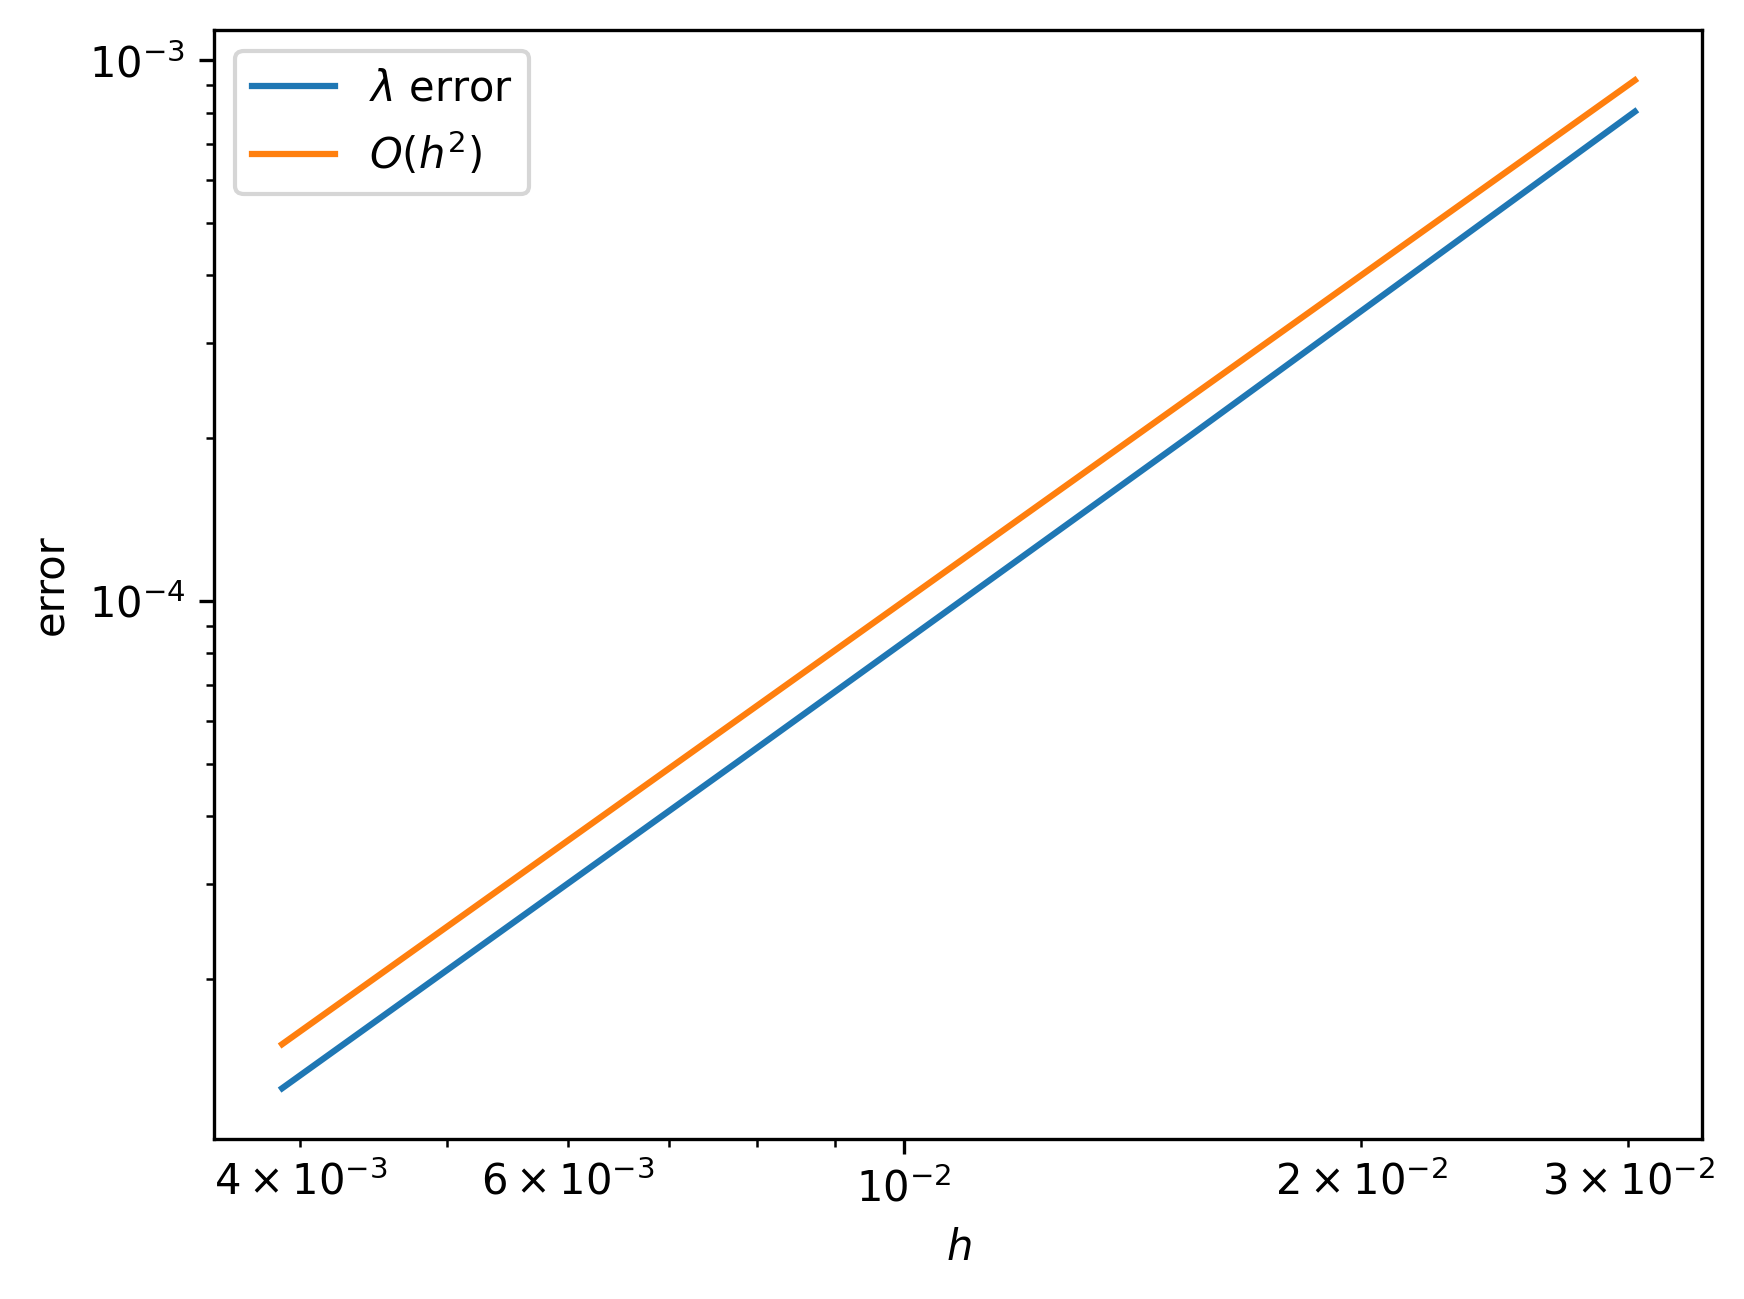
\includegraphics[width=0.5\linewidth]{convergence_test.png}
    \caption{Convergence test for the $1$D Laplace eigenvalue problem. The plot is a log-log plot of the absolute error in the smallest eigenvalue computed using piecewise linear elements on a uniform triangular mesh, plotted against the number of mesh elements $N$ (the mesh has $N \times N$ elements). As expected, we observe approximately second-order convergence.}
    \label{conv test}
\end{figure}


We note that in this setting, the eigenvalues are approximated from above:
\begin{equation}
\lambda^{(k)} \le \lambda_h^{(k)} \le \lambda^{(k)} + C(k) h^2.
\end{equation}
Furthermore, since eigenmodes are unique up to scalar multiples, we need to be careful when computing $\| u^{(k)}  - u_h^{(k)} \|_V.$ To overcome this issue, we first normalize the computed eigenmode. To overcome any sign discrepancies, we choose the sign to match the sign of $u^{(k)}$ (ensure their scalar product is positive).


Now, let $V_h$ be the space of continuous piecewise polynomials of degree at most $p$ that vanish at the endpoints of the interval (standard conforming $P^p$ elements). Then, our convergence results are
\begin{equation}
    \| u^{(k)}  - u_h^{(k)} \|_V = O(h^p)
\end{equation}
and
\begin{equation}
    | \lambda^{(k)} - \lambda_h^{(k)} | = O(h^{2p}).
\end{equation}

\subsection{On a Square Domain}

Let $\Omega = (0, \pi) \times (0, \pi).$ We want to find the eigenvalues $\lambda$ and the eigenfunctions $u \ne 0$ such that
\begin{equation}\label{strong 2D}
\begin{aligned}
    - \nabla^2 u &= \lambda u, \qquad (x,y) \in \Omega,\\
    u &= 0 \qquad \forall \, (x, y) \in \partial \Omega.
\end{aligned}
\end{equation}
Here, the exact eigenvalues are
\begin{equation}
\lambda_{m,n} = m^2 + n^2,
\end{equation}
with eigenfunctions
\begin{equation}
u_{m,n} = \sin(mx) \sin(ny), 
\end{equation}
for $m, n \in \mathbb{N}_1.$


Let $V = H_0^1(\Omega).$ As before, the variational formulation of \eqref{strong 2D} is: find a $\lambda \in \mathbb{R}$ and a nonzero $u \in V$ such that
\begin{equation}
\int_{\Omega} \nabla u \cdot \nabla v \, dx dy = \lambda \int_{\Omega} u v \, dxdy,
\end{equation}
for all $v \in V.$


To discretize, we solve for a solution in a finite-dimensional subspace $V_h \subset V,$ namely, the space of continuous piecewise linear finite elements. Thus, we want to find a $\lambda_h \in \mathbb{R}$ and a nonzero $u_h \in V_h$ such that
\begin{equation}
    \int_{\Omega} \nabla u_h \cdot \nabla v \, dx dy = \lambda_h \int_{\Omega} u_h v \, dxdy, 
\end{equation}
for all $v \in V_h.$




As in one dimension, the eigenvalues are approximated from above. Similarly, in one dimension we saw that $| \lambda^{(k)} - \lambda_h^{(k)} | = O(k^4 h^2).$ Thus, the error increases with the rank of the eigenvalues. This is again observed in 2D.

Consider the double eigenvalue $\lambda = 5,$ whose eigenspace is two-dimensional. The numerical method will approximate $\lambda = 5$ twice, with two eigenmodes $u_h^{(1)}$ and $u_h^{(2)}$. However, because the exact eigenspace is two-dimensional, the computed eigenmodes need not converge to the particular basis functions, say $u_1$ and $u_2.$ Rather, they can converge to any linear combination of $u_1$ and $u_2.$ 

Therefore, for multiple eigenvalues, to compute the error in the computed eigenmodes, we compare the computed eigenspace to the exact eigenspace rather than the individual eigenfunctions. For example, for $\lambda = 5$, we expect constants $\alpha_1(h),$ $\alpha_2(h),$ $\beta_1(h),$ and $\beta_2(h)$ such that
\begin{equation}
    \| u_{1} - \alpha_1(h) u_h^{(1)} - \beta_1(h) u_h^{(2)} \|_{V} = O(h)
\end{equation}
and
\begin{equation}
   \| u_{2} - \alpha_2(h) u_h^{(1)} - \beta_2(h) u_h^{(2)} \|_{V} = O(h), 
\end{equation}
where $h$ is the maximum diameter of any element of the mesh\footnote{Is this the correct definition of $h$ in this context?}. The dependence of $\alpha_1(h),$ $\alpha_2(h),$ $\beta_1(h),$ and $\beta_2(h)$ on the mesh 
reflects the nonuniqueness of the computed eigenbasis for a multiple eigenvalue. In particular, as the mesh varies, the computed eigenmodes may converge to different linear combinations of $u_1$ and $u_2.$  

To illustrate this mesh-dependence, we first approximate the eigenvalues and eigenfunctions of \eqref{strong 2D} on a sequence of unstructured meshes. These results are shown in Figure \ref{unstructured}. 

\begin{figure}[htbp]
    \centering

    \begin{subfigure}{1.0\textwidth}
        \centering
        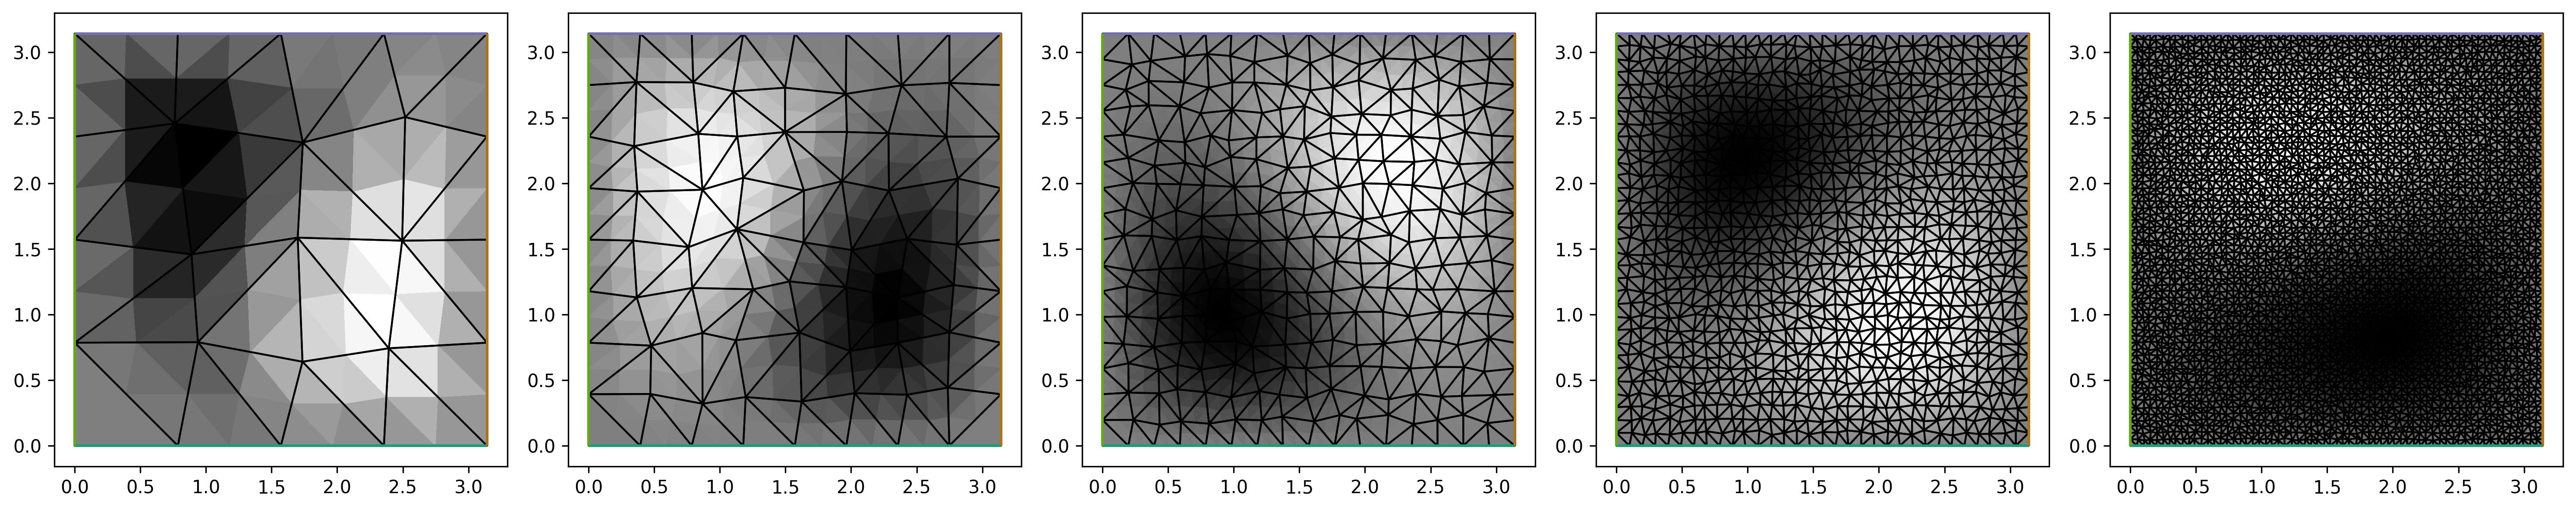
\includegraphics[width=\textwidth]{unstructured_u1h.png}
        \caption{Computed eigenmodes for the first approximation of $\lambda = 5$ on an unstructured mesh sequence.}
        \label{fig:diag-one}
    \end{subfigure}

    \vspace{1em}

    \begin{subfigure}{1.0\textwidth}
        \centering
        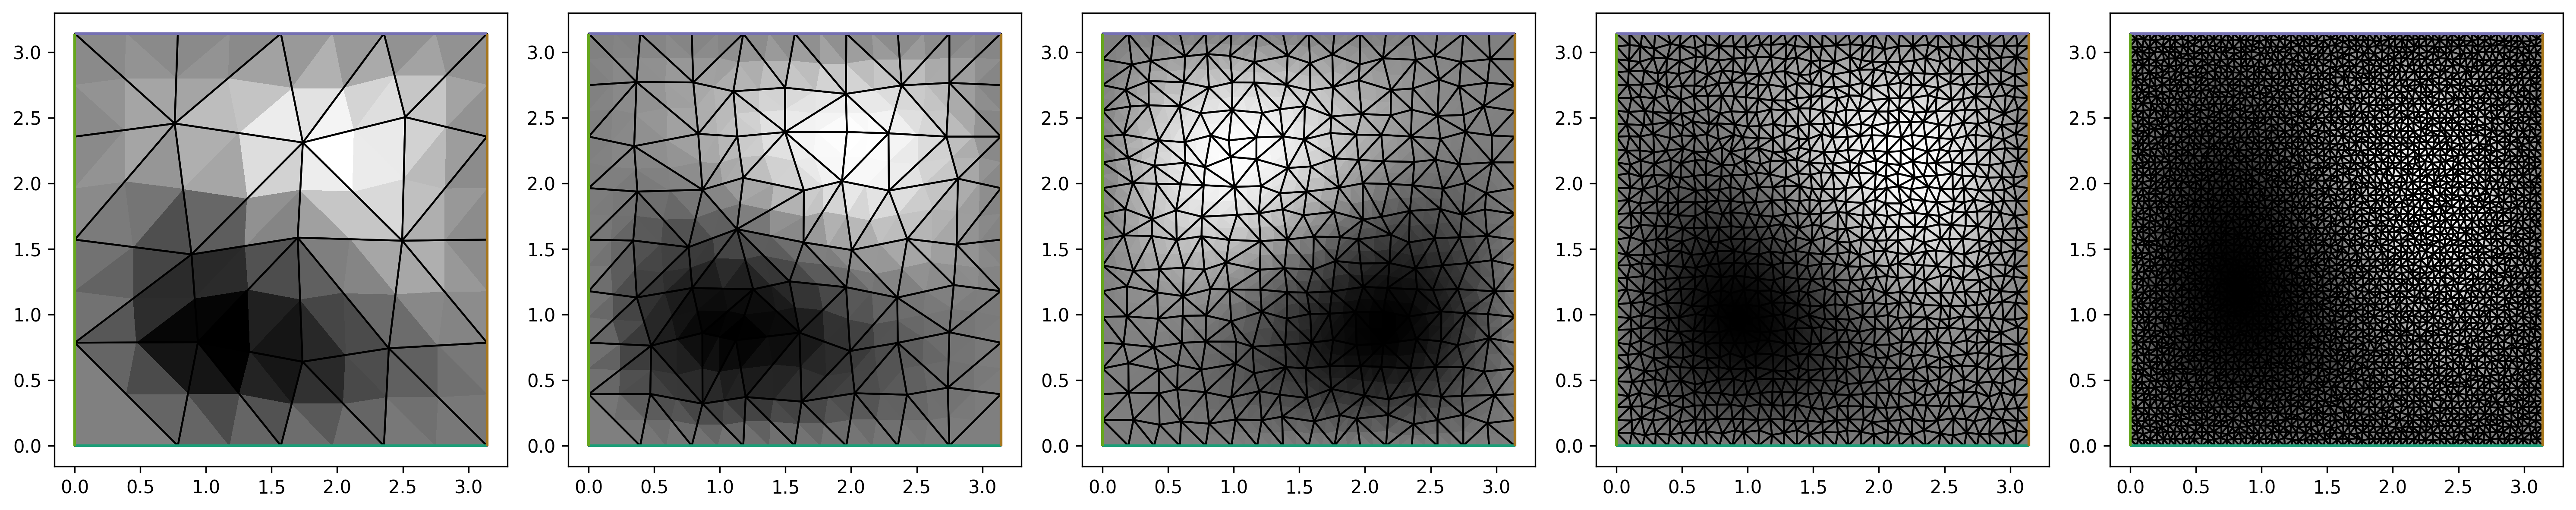
\includegraphics[width=\textwidth]{unstructured_u2h_png.png}
        \caption{Computed eigenmodes for the second approximation of $\lambda = 5$ on an unstructured mesh sequence.}
        \label{fig:diag-two}
    \end{subfigure}

    \vspace{1em}

    \begin{subfigure}{0.4\textwidth}
        \centering
        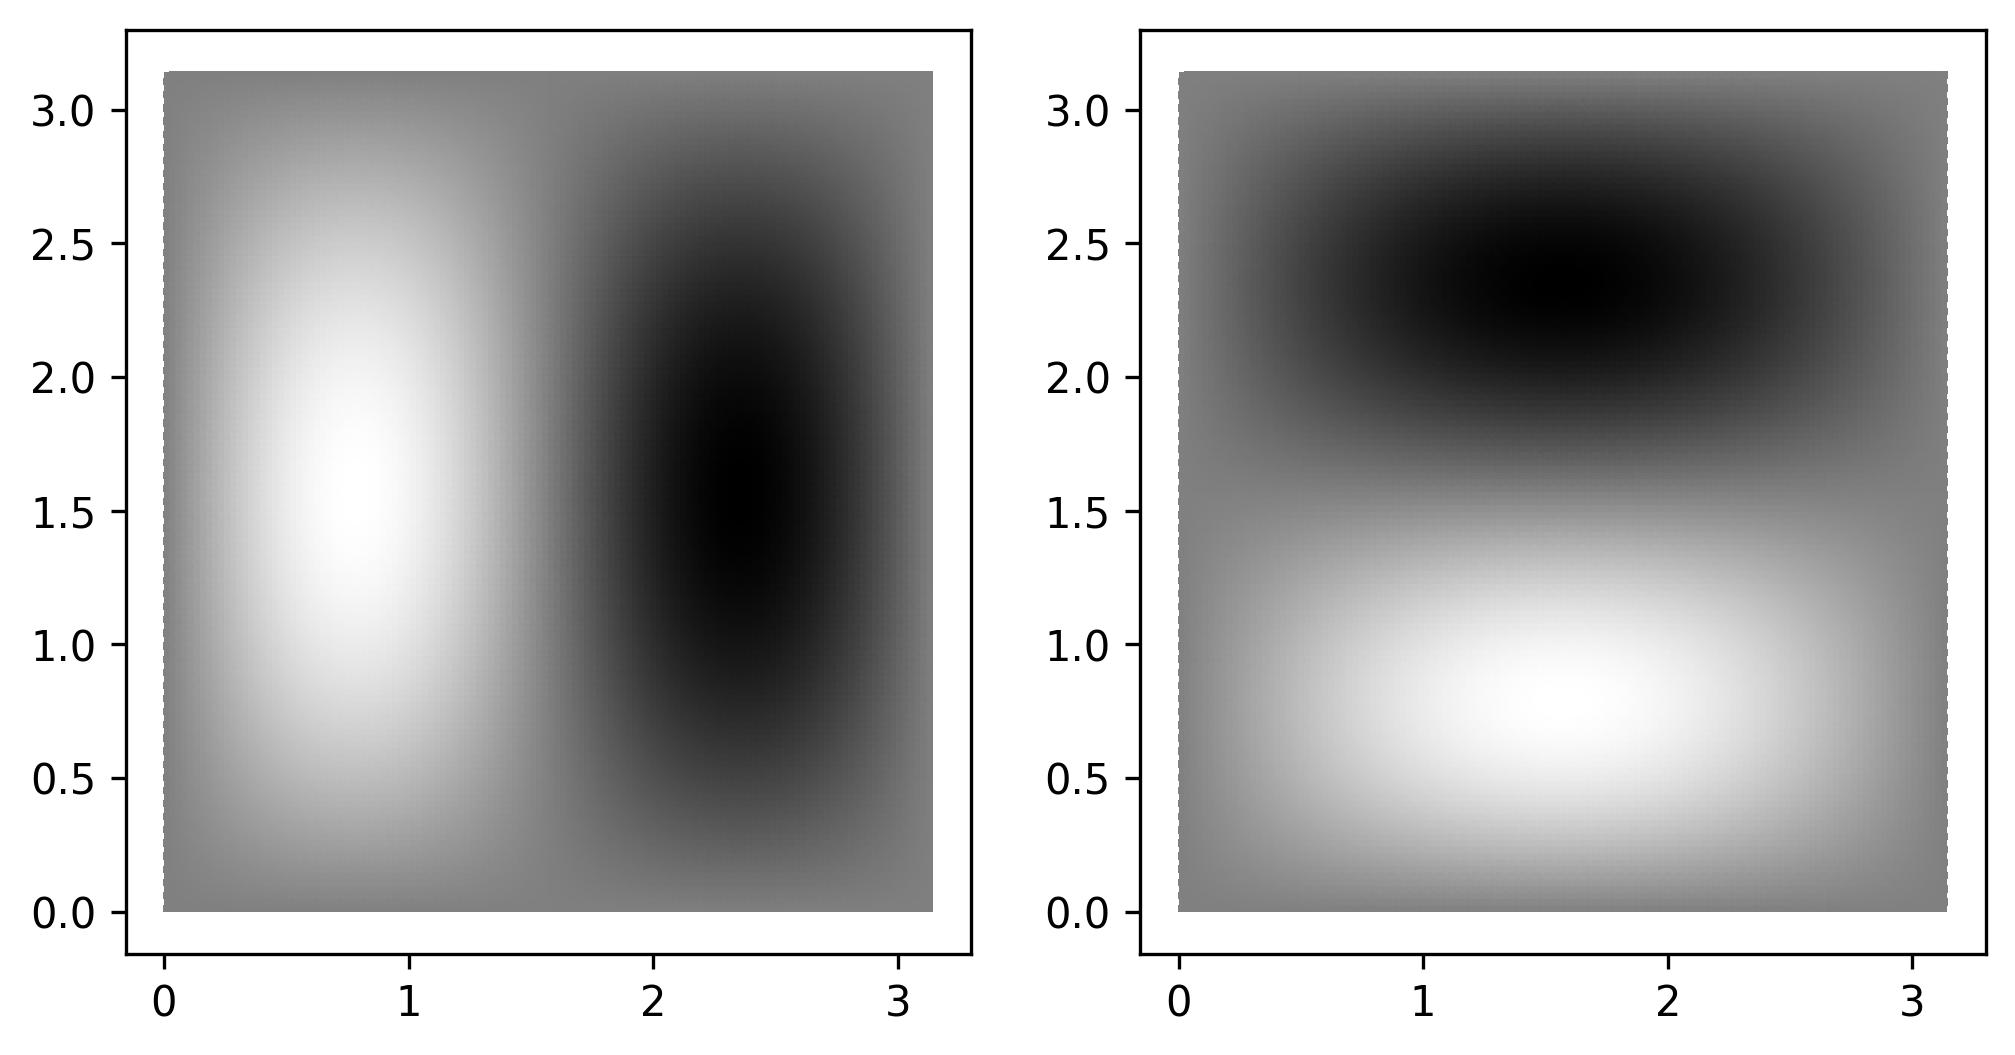
\includegraphics[width=\textwidth]{unstructured_u12.png}
        \caption{The exact eigenfunctions.}
        \label{fig:eigenfunction-comparison}
    \end{subfigure}

    \caption{The computed eigenmodes for both approximations of $\lambda = 5$ on sequences of unstructured meshes.}
    \label{unstructured}
\end{figure}

The situation is similar for structured uniform meshes, where we see an improvement in the computed convergence rates because the mesh is uniform. The results are shown in Figure \ref{structured}, where the computed eigenmodes are visibly influenced by the preferred diagonal direction of the mesh.

\begin{figure}[htbp]
    \centering

    \begin{subfigure}{1.0\textwidth}
        \centering
        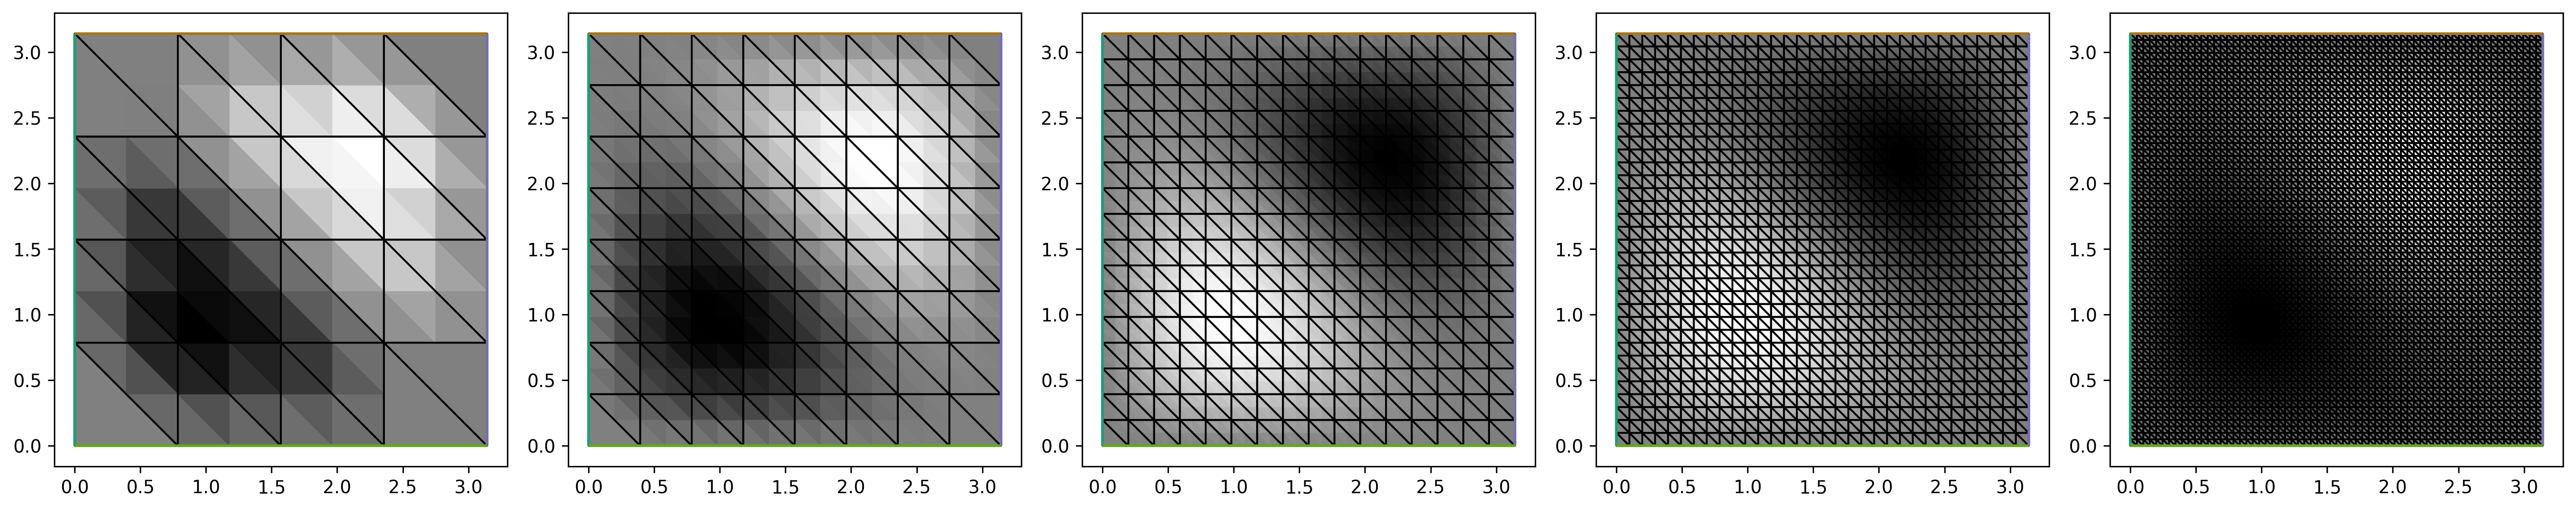
\includegraphics[width=\textwidth]{structured_u1h.png}
        \caption{Computed eigenmodes for the first approximation of $\lambda = 5$ on a uniform structured mesh sequence.}
        \label{fig:diag-one}
    \end{subfigure}

    \vspace{1em}

    \begin{subfigure}{1.0\textwidth}
        \centering
        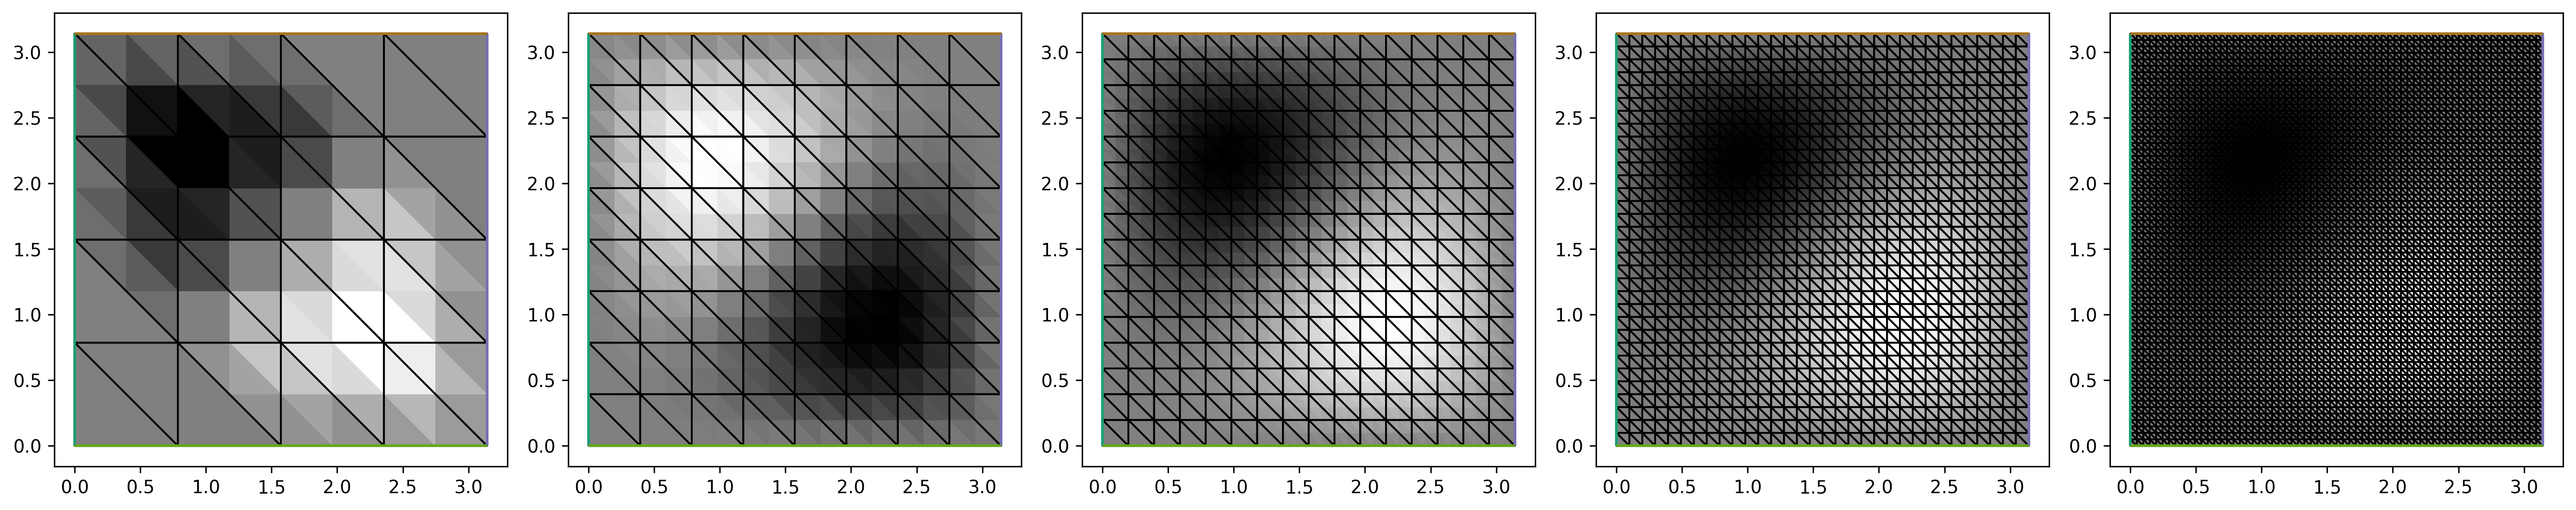
\includegraphics[width=\textwidth]{structured_u2h.png}
        \caption{Computed eigenmodes for the second approximation of $\lambda = 5$ on a unfiorm structured mesh sequence.}
        \label{fig:diag-two}
    \end{subfigure}

    % \vspace{1em}

    % \begin{subfigure}{0.4\textwidth}
    %     \centering
    %     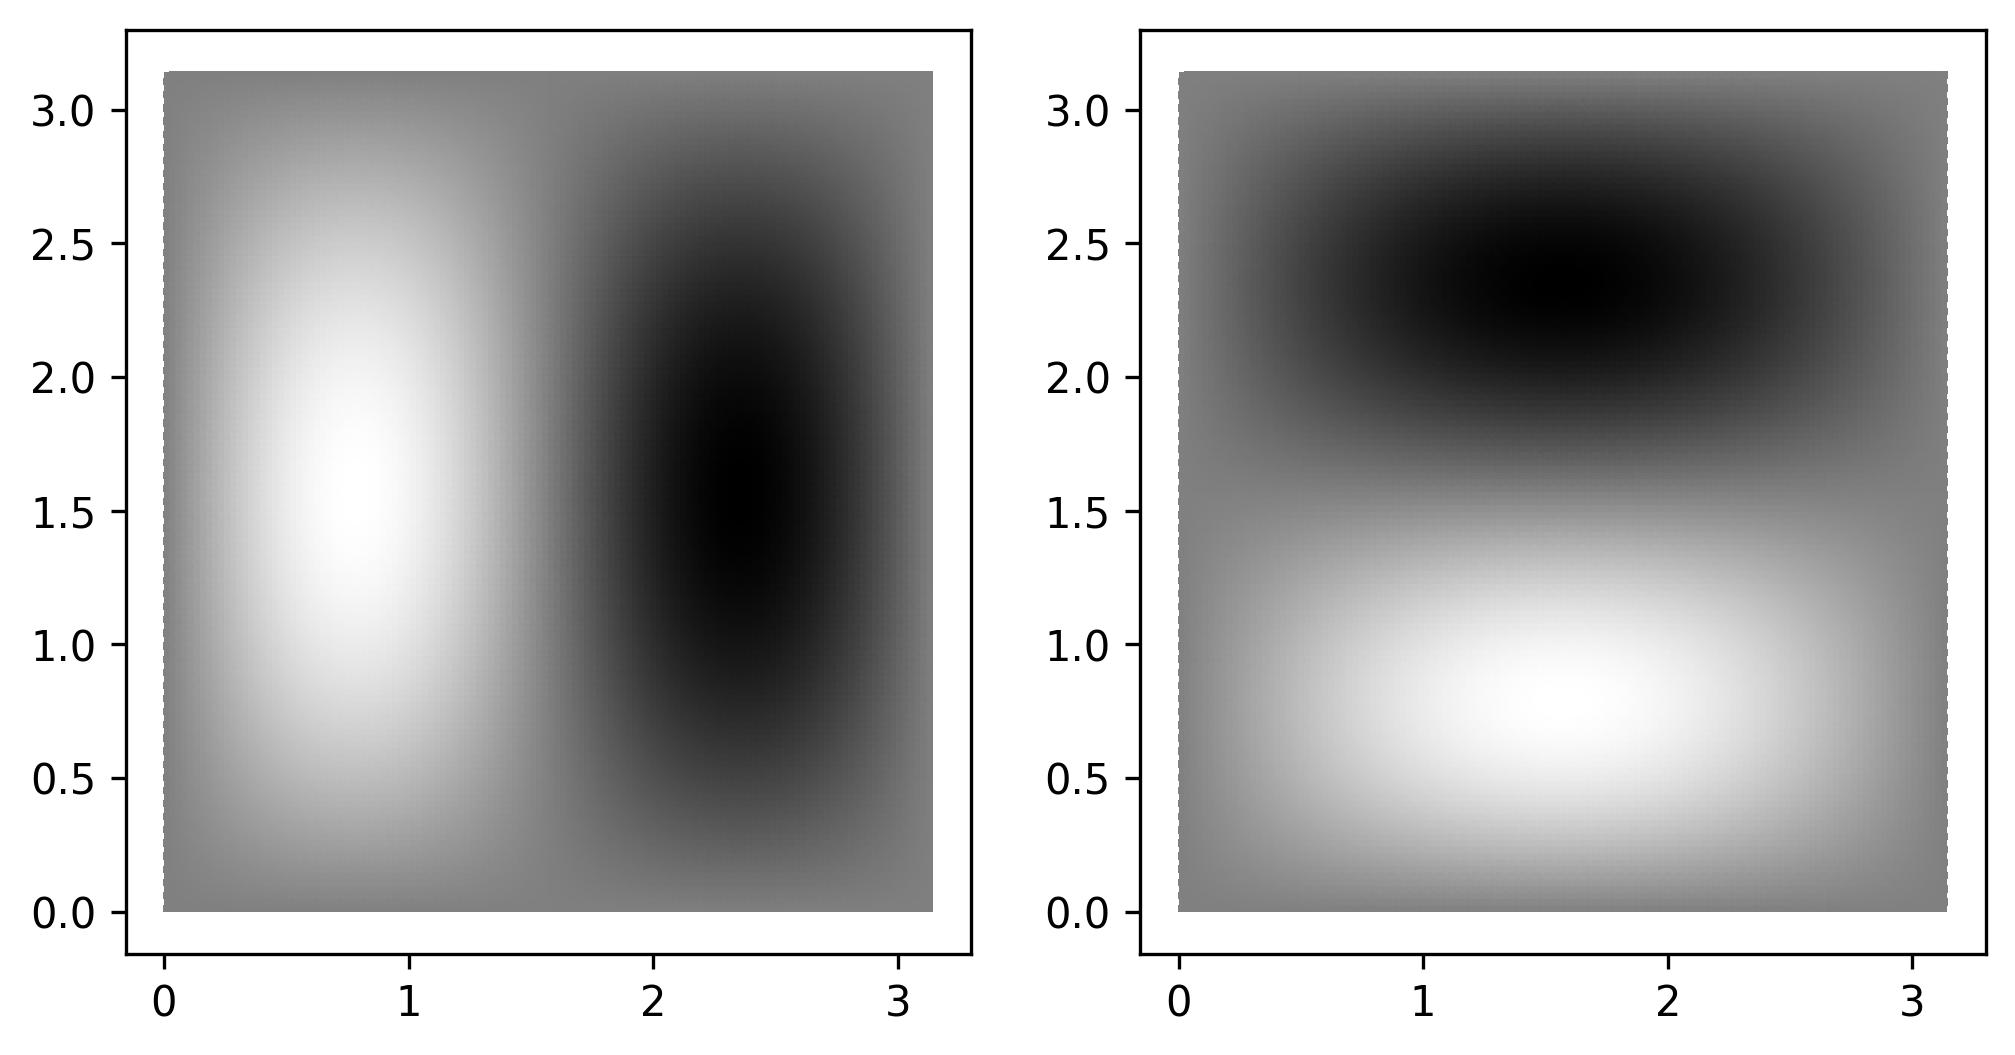
\includegraphics[width=\textwidth]{structured_u12.png}
    %     \caption{The exact eigenfunctions.}
    %     \label{fig:eigenfunction-comparison}
    % \end{subfigure}

    \caption{The computed eigenmodes for both approximations of $\lambda = 5$ on sequences of uniform structured meshes.}
    \label{structured}
\end{figure}



To further explore this mesh-dependence, we take another uniform grid, but now cut each square along the opposite diagonal direction. The eigenvalues are the same as before. 
However, as shown in Figure \ref{reverse}, the eigenfunctions change. This behaviour change is attributed to the change in the preferred diagonal direction of the mesh. As a result, the discrete problem selects different linear combinations inside the same eigenspace. This result is not surprising since the problem is invariant under the change of variables induced by the symmetry about the line $y=\pi-x.$
% This result is expected since the new mesh is just a reflected/rotated version of the old one.

\begin{figure}[htbp]
    \centering

    \begin{subfigure}{1.0\textwidth}
        \centering
        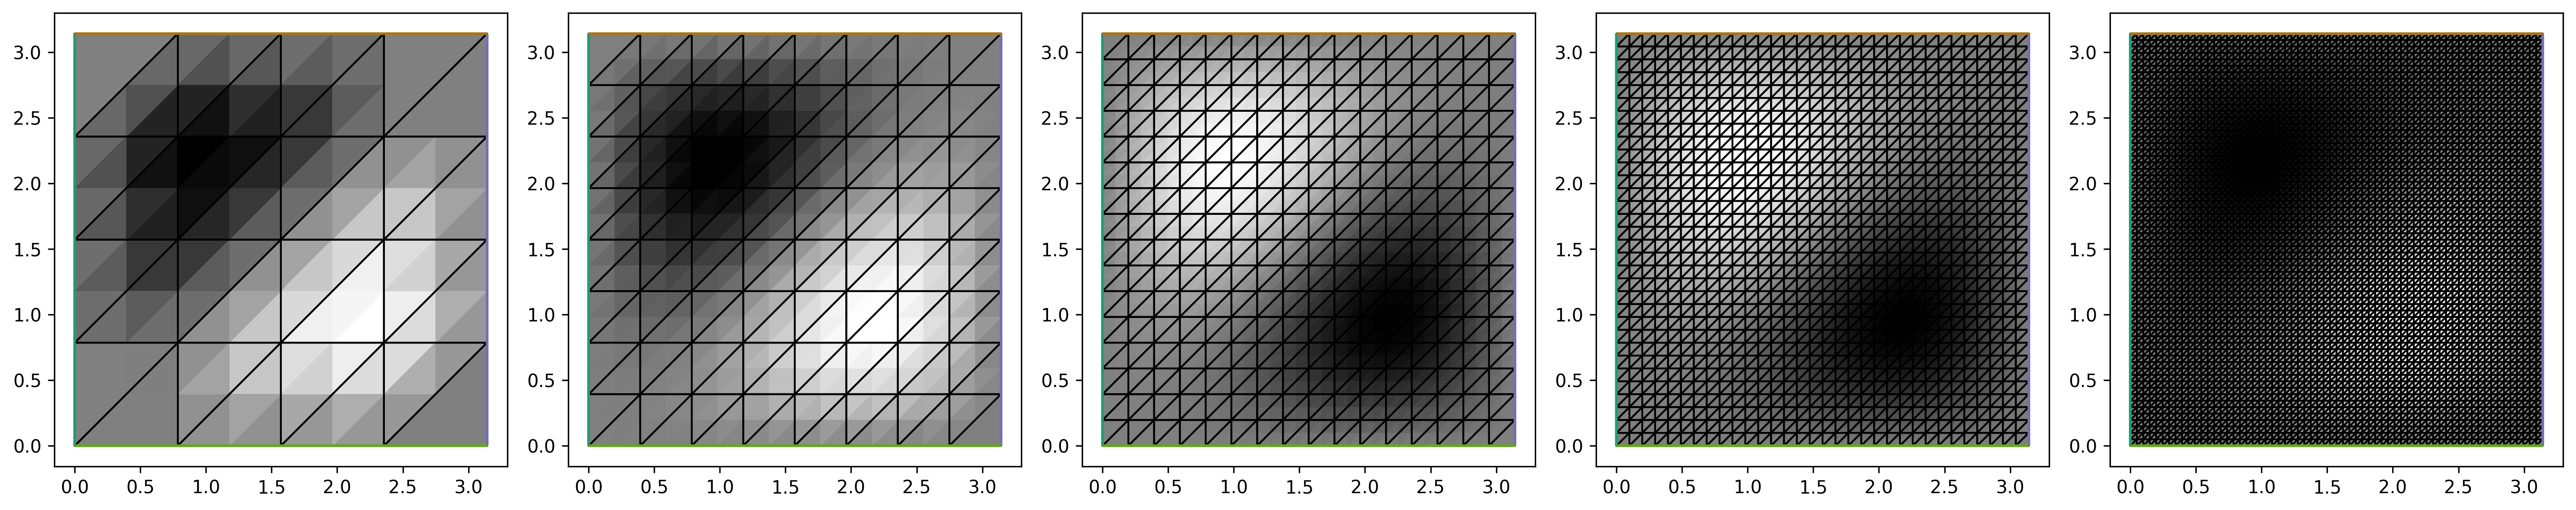
\includegraphics[width=\textwidth]{reverse_u1h.png}
        \caption{Computed eigenmodes for the first approximation of $\lambda = 5$ on a uniform structured mesh sequence (reverse orientation).}
        \label{fig:diag-one}
    \end{subfigure}

    \vspace{1em}

    \begin{subfigure}{1.0\textwidth}
        \centering
        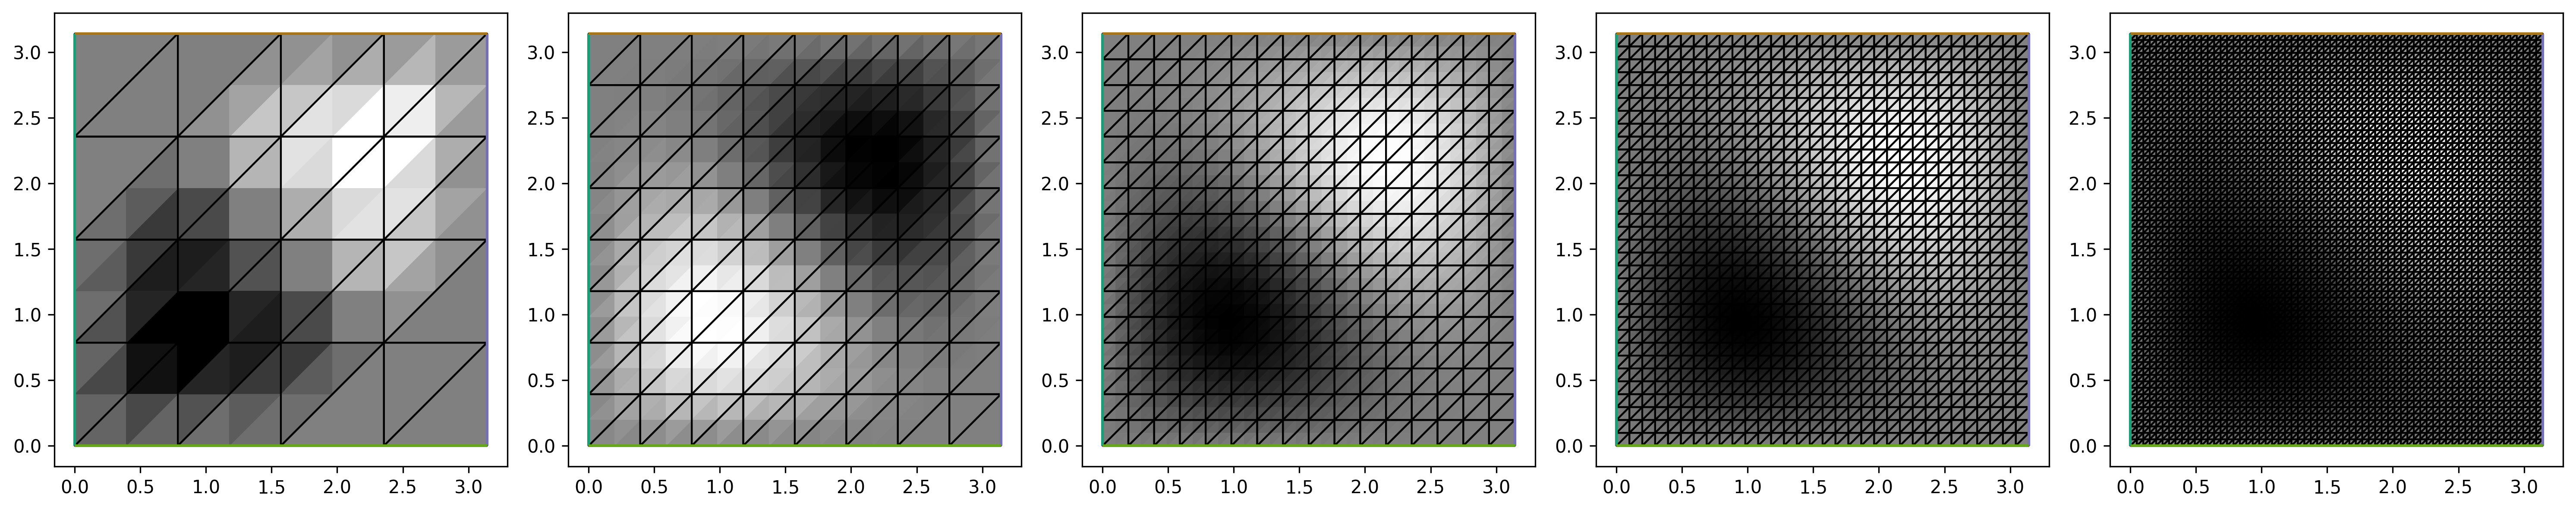
\includegraphics[width=\textwidth]{reverse_u2h.png}
        \caption{Computed eigenmodes for the second approximation of $\lambda = 5$ on a unfiorm structured mesh sequence (reverse orientation).}
        \label{fig:diag-two}
    \end{subfigure}

    % \vspace{1em}

    % \begin{subfigure}{0.4\textwidth}
    %     \centering
    %     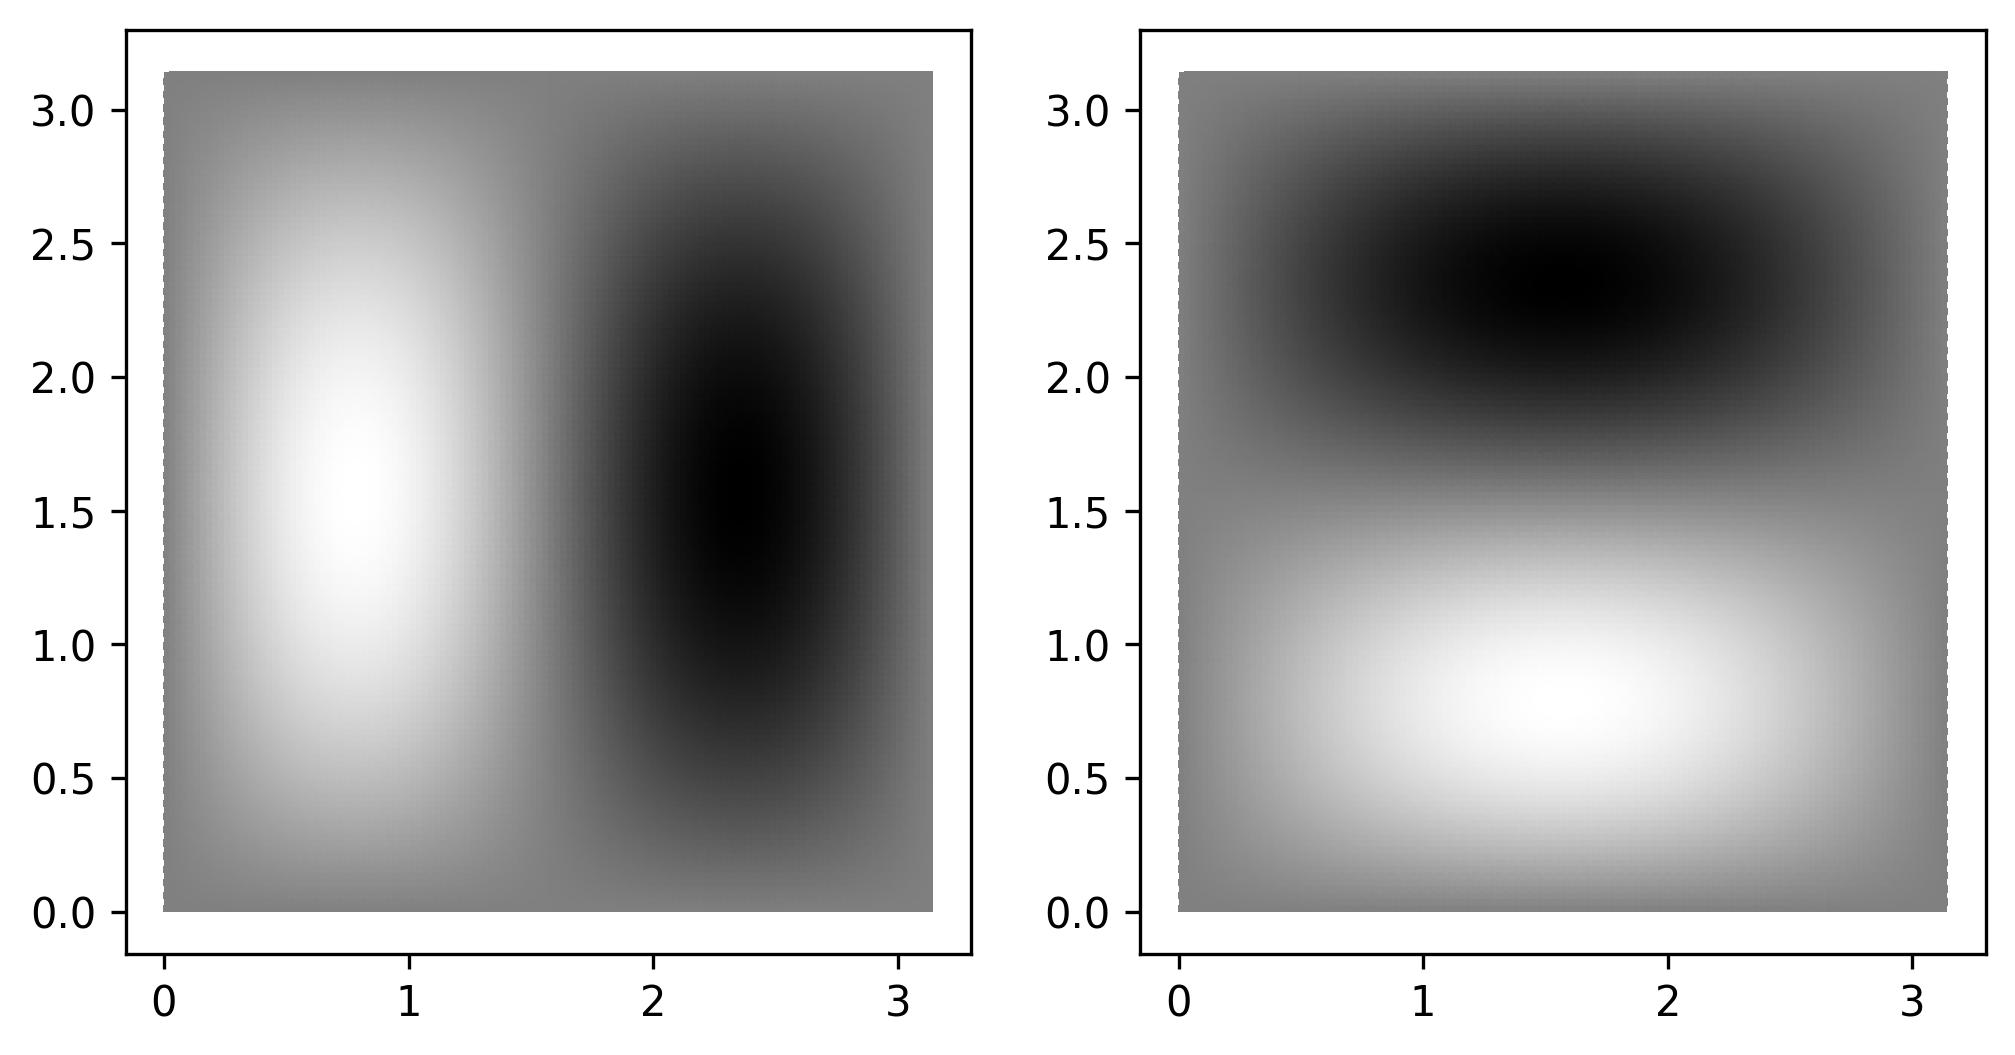
\includegraphics[width=\textwidth]{reverse_u12.png}
    %     \caption{The exact eigenfunctions.}
    %     \label{fig:eigenfunction-comparison}
    % \end{subfigure}

    \caption{The computed eigenmodes for both approximations of $\lambda = 5$ on sequences of uniform structured meshes (reverse orientation).}
    \label{reverse}
\end{figure}

Next, we consider a sequence of criss-cross meshes. The results of this example are shown in Table \ref{table criss cross}. Notice that the additional symmetry of these meshes manifests as coinciding approximations of some of the repeated eigenvalues. For example, $\lambda = 5,$ $\lambda = 10,$ and $\lambda = 13$ are approximated by discrete eigenvalues that are the same up to machine precision. However, this is not the case for the approximations of $\lambda = 17$ on the coarsest mesh. This occurs because the ninth computed eigenvalue, $\lambda_h^{(9)},$ is a bad approximation of $\lambda = 18$ instead of $\lambda = 17.$ This is supported by the comparison between the computed eigenmode for $\lambda_h^{(9)}$ and the exact eigenfunction for $\lambda = 18$ in Figure \ref{compare}. Thus, this example should be taken as a cautionary tale: when the discretization is too coarse, the order of the computed eigenvalues need not be in one-to-one correspondence with the exact eigenvalues.

% \begin{table}[htbp]
\begin{table}[htbp]
\centering
\caption{Computed eigenvalues on the sequence of criss-cross meshes. Given in parentheses are the observed convergence rates. Note that I have not explained what $N$ is!}
\label{table criss cross}
\resizebox{\textwidth}{!}{%
\begin{tabular}{c|ccccc}
\toprule
Exact & \multicolumn{5}{c}{Computed (rate)} \\
\cmidrule(lr){2-6}
 & $N=4$ & $N=8$ & $N=16$ & $N=32$ & $N=64$ \\
\midrule
$2$  & $2.0880$  & $2.0216\ (2.0)$  & $2.0054\ (2.0)$  & $2.0013\ (2.0)$  & $2.0003\ (2.0)$ \\
$5$  & $5.6811$  & $5.1651\ (2.0)$  & $5.0408\ (2.0)$  & $5.0102\ (2.0)$  & $5.0025\ (2.0)$ \\
$5$  & $5.6811$  & $5.1651\ (2.0)$  & $5.0408\ (2.0)$  & $5.0102\ (2.0)$  & $5.0025\ (2.0)$ \\
$8$  & $9.4962$  & $8.3521\ (2.1)$  & $8.0863\ (2.0)$  & $8.0215\ (2.0)$  & $8.0054\ (2.0)$ \\
$10$ & $12.9691$ & $10.7578\ (2.0)$ & $10.1865\ (2.0)$ & $10.0464\ (2.0)$ & $10.0116\ (2.0)$ \\
$10$ & $12.9691$ & $10.7578\ (2.0)$ & $10.1865\ (2.0)$ & $10.0464\ (2.0)$ & $10.0116\ (2.0)$ \\
$13$ & $17.1879$ & $14.0237\ (2.0)$ & $13.2489\ (2.0)$ & $13.0617\ (2.0)$ & $13.0154\ (2.0)$ \\
$13$ & $17.1879$ & $14.0237\ (2.0)$ & $13.2489\ (2.0)$ & $13.0617\ (2.0)$ & $13.0154\ (2.0)$ \\
$17$ & $25.1471$ & $19.3348\ (1.8)$ & $17.5733\ (2.0)$ & $17.1423\ (2.0)$ & $17.0355\ (2.0)$ \\
$17$ & $38.9073$ & $19.3348\ (3.2)$ & $17.5733\ (2.0)$ & $17.1423\ (2.0)$ & $17.0355\ (2.0)$ \\
$18$ & $38.9073$ & $19.8363\ (3.5)$ & $18.4405\ (2.1)$ & $18.1089\ (2.0)$ & $18.0271\ (2.0)$ \\
$20$ & $38.9073$ & $22.7243\ (2.8)$ & $20.6603\ (2.0)$ & $20.1634\ (2.0)$ & $20.0407\ (2.0)$ \\
$20$ & $38.9073$ & $22.7243\ (2.8)$ & $20.6603\ (2.0)$ & $20.1634\ (2.0)$ & $20.0407\ (2.0)$ \\
$25$ & $38.9073$ & $28.7526\ (1.9)$ & $25.8940\ (2.1)$ & $25.2202\ (2.0)$ & $25.0548\ (2.0)$ \\
$25$ & $38.9073$ & $28.7526\ (1.9)$ & $25.8940\ (2.1)$ & $25.2202\ (2.0)$ & $25.0548\ (2.0)$ \\
\midrule
DOF & $25$ & $113$ & $481$ & $1985$ & $8065$ \\
\bottomrule
\end{tabular}%
}
\end{table}



\begin{figure}
    \centering
    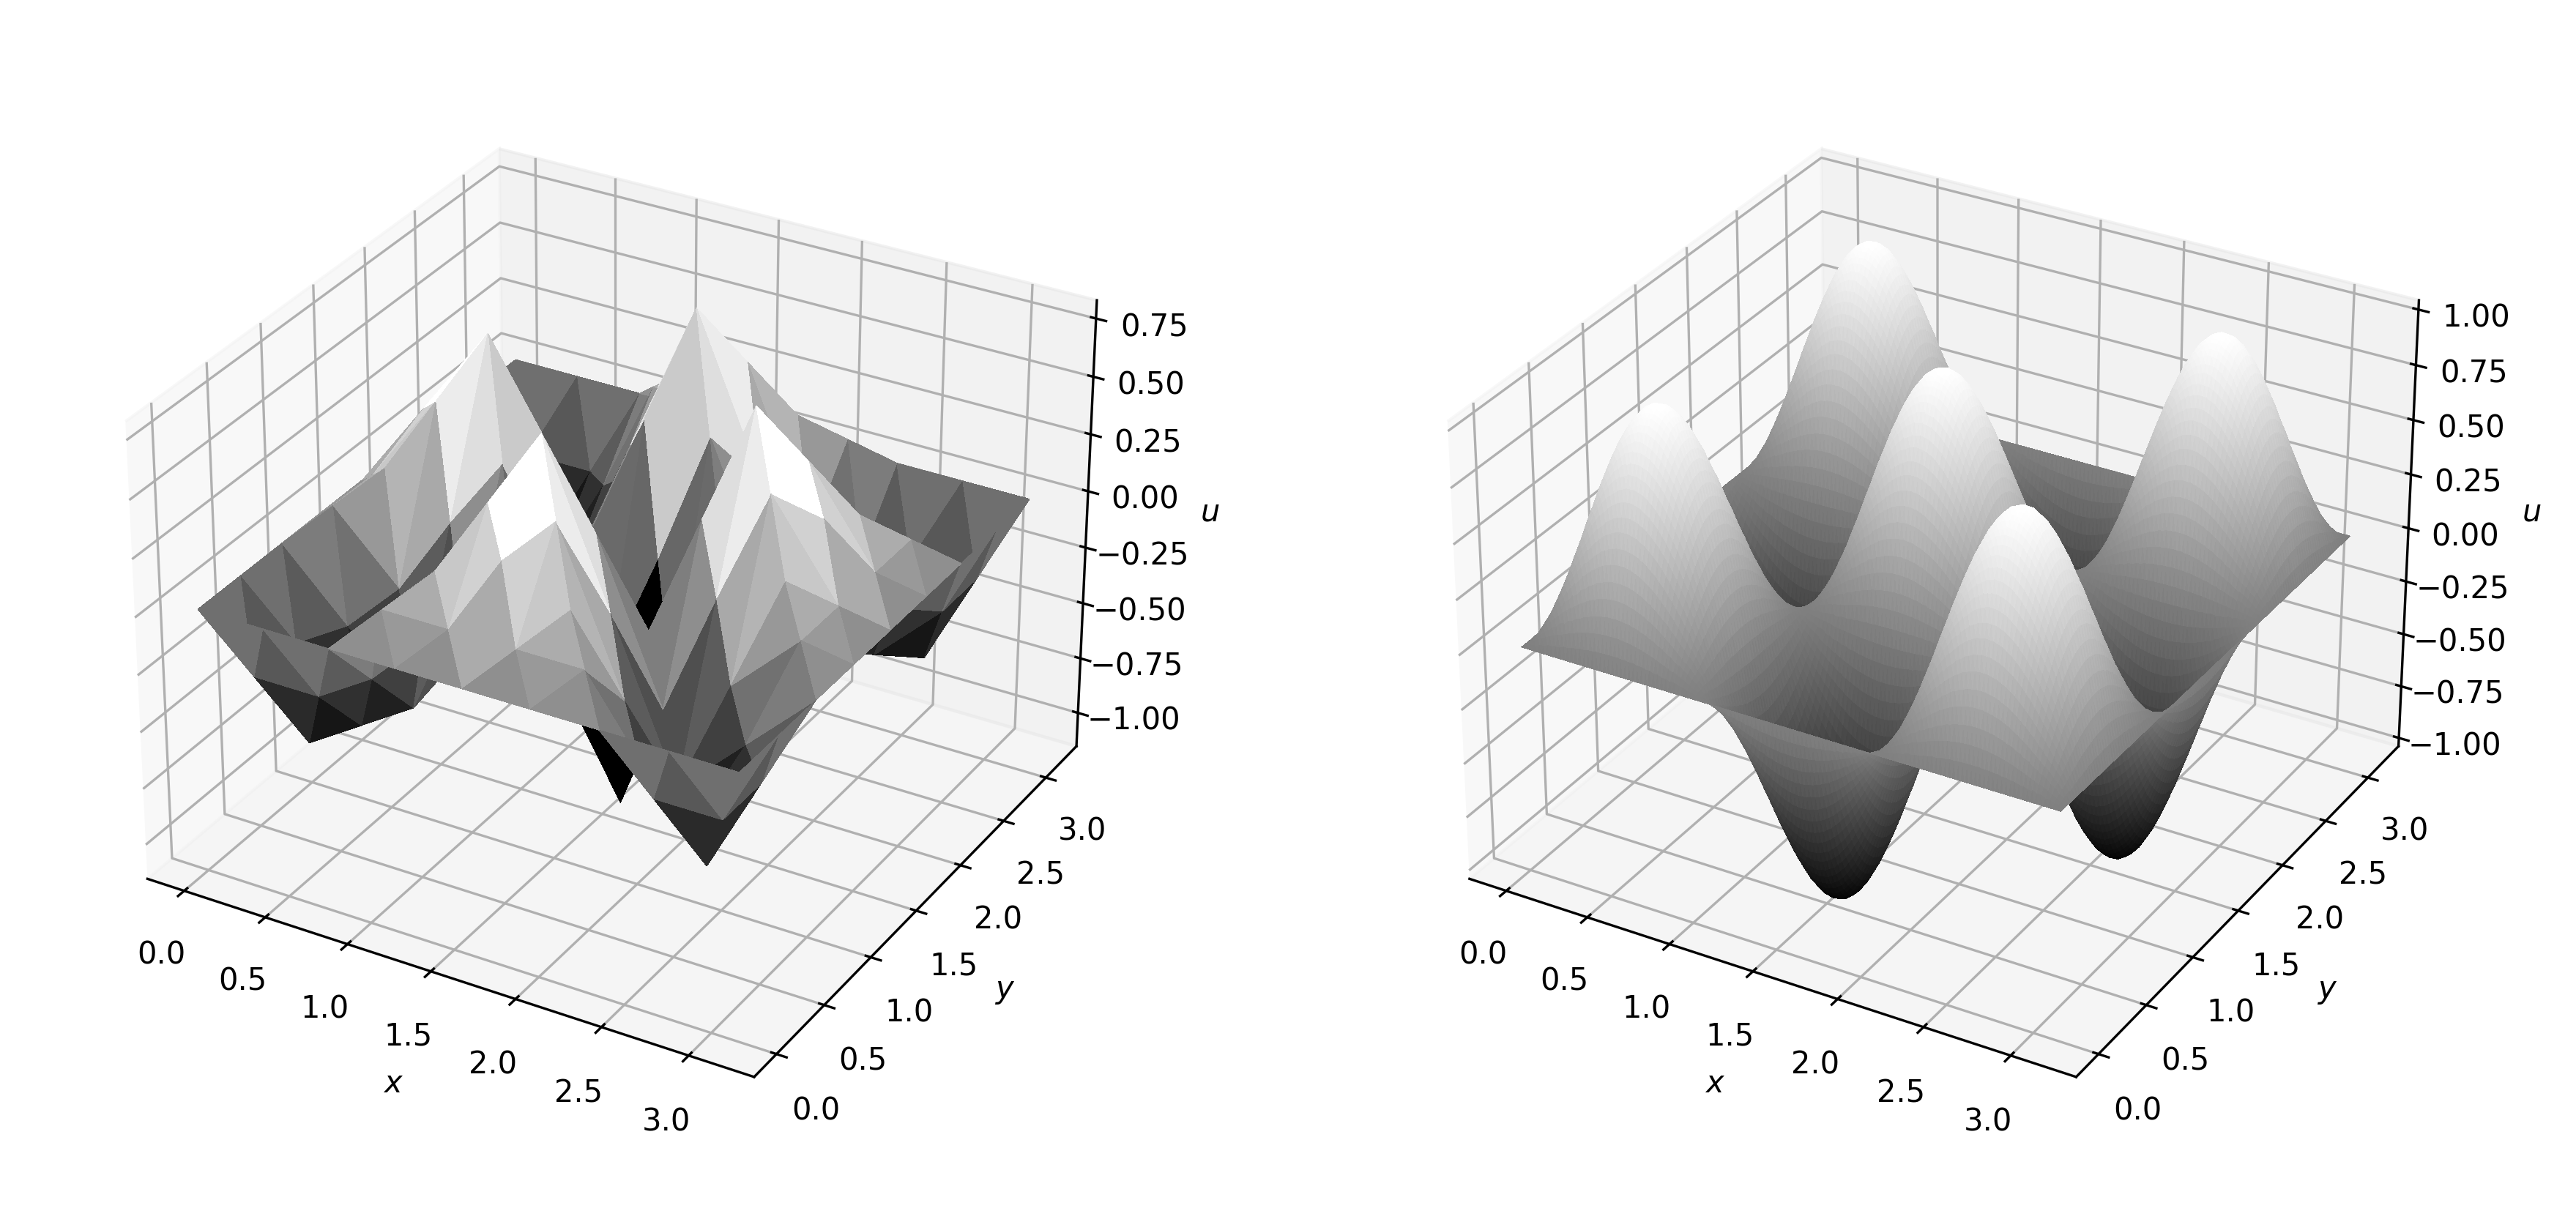
\includegraphics[width=1.0\linewidth]{eigenfunc_comparison.png}
    \caption{Comparing the computed eigenmode for the ninth computed eigenvalue to the exact eigenfunction for $\lambda = 18,$ namely, $u(x, y) = \sin(3x)\sin(3y).$}
    \label{compare}
\end{figure}


\subsection{On an L-Shaped Domain}

\section{Maxwell Eigenvalue Problem}



\end{document}
